\subsubsection{Endpoint para realizar una solicitud de puntos}
Este es el último endpoint que utiliza esta sección.

Para poder realizar una solicitud de puntos, el usuario debe llenar un formulario donde se le solicita que indique que productos compró, la cantidad y suba una imagen que sea evidencia de esta compra.

Es en este endpoint donde se integra un nuevo servicio de Amazon: Amazon Simple Storage Service (Amazon S3) que proporciona los llamados ``buckets'' para almacenar archivos. Para poder utilizar Amazon S3, es necesario instalar la librería para el lenguaje de programación que se esté utilizando (que en este caso es JavaScript) que proporciona Amazon. Una vez instalada, en un archivo específico para esta configuración, se importa esta librería para acceder a la clase necesaria para la configuración. Para una configuración básica sólo se requieren de tres datos: la región donde está ubicado el bucket, una llave de acceso y una llave de acceso secreta; esta información se obtiene a través de la cuenta de AWS.

El objeto que se obtiene como resultado de esta configuración es el siguiente (Ver Figura 9):

    \begin{figure}[H]
        \begin{center}
            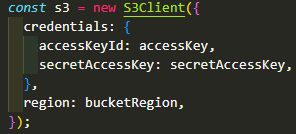
\includegraphics[scale=0.85]{img/actividades/detalles-campanias/objeto-as3.png}
            \caption{Objeto de configuración de Amazon S3.}
            \label{fig:objeto-as3}
        \end{center}
    \end{figure}

Una vez hecha la configuración de Amazon S3, se puede continuar con el procesamiento de los datos.

Como se mencionó anteriormente, el usuario llena un formulario para enviar la información de su solicitud de puntos. El Backend no recibe esta información en formato JSON, como se hizo en el endpoint de inicio de sesión, esta vez la recibe como FormData, y esto es porque el usuario debe subir un archivo, y este formato es el más adecuado para estas situaciones.

Este FormData está formado por dos pares llave/valor: uno con toda la información del formulario (que esta sí está en formato JSON) y otro con el archivo que se va a subir.

El controlador recibe la petición con el FormData y se extraen el ID del usuario, el archivo y la información del formulario. Todo esto, posteriormente, es enviado al servicio.

El servicio es el que se encarga de procesar toda esta información. Primero se trabaja con el archivo, se obtiene la extensión del archivo y se verifica si está entre las permitidas; si no es permitido, se detiene el proceso de subida del archivo y se manda un error, si es permitido, avanza con el proceso. Lo siguiente que se hace es generar una ruta para almacenar la imagen en el bucket, esta ruta tiene la siguiente estructura: ``Campania/idCampania/Pruebas/idUsuario''. Posteriormente se crea un nombre único para el archivo mediante un algoritmo de encriptación que retorna una cadena de caracteres aleatorios, este nombre se anexa al final de la ruta creada anteriormente. Para subir el archivo, se crea un objeto con los parámetros que requiere Amazon S3 para subir un archivo a un bucket, este objeto tiene la siguiente estructura (Ver Figura 10):

    \begin{figure}[H]
        \begin{center}
            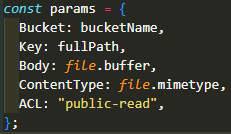
\includegraphics[scale=0.85]{img/actividades/detalles-campanias/params-as3.png}
            \caption{Parámetros para subir un archivo a un bucket.}
            \label{fig:params-as3}
        \end{center}
    \end{figure}

Los parámetros significan lo siguiente: 
    \begin{itemize}
        \item Bucket: Nombre del bucket donde se guardará el archivo.
        \item Key: La ruta donde se guardará el archivo.
        \item Body: El contenido del archivo que se subirá.
        \item ContentType: El formato del archivo.
        \item ACL: La lista de control de acceso para indicar quien podrá ver el archivo y quien no.
    \end{itemize}

Estos parámetros se envían al método correspondiente al objeto que se creó anteriormente en el archivo de configuración, y de esta manera el archivo quedará subido.

El siguiente paso es insertar toda la información en la tabla de la base de datos. Una gran parte de los campos requeridos ya venían en el FormData, por lo que sólo es cuestión de extraerlos y colocarlos en un nuevo objeto que se envía al método encargado de insertar los datos, el único campo nuevo que se debe crear es la URL completa de la imagen, es decir, la URL que contiene tanto el servidor del bucket y la ruta que se creó anteriormente. Este nuevo campo se anexa al objeto y finalmente se envía para insertar esos datos.

Este método retorna el ID del nuevo registro que se creó, este se almacena en una variable para utilizarlo posteriormente. Cabe mencionar que, hasta el momento de la redacción de este reporte, las solicitudes son aceptadas automáticamente, esto por petición de la empresa, lo ideal es que en un futuro las solicitudes pasen por su debido proceso de revisión.

También se deben de insertar los detalles de la solicitud, esto es los productos que se compraron y la cantidad. Al igual que los datos de la inserción anterior, estos detalles también se obtienen del FormData, sólo es cuestión de extraerlos y anexarlos al nuevo objeto que se va a enviar; a este nuevo objeto también se le va a anexar el ID que se almacenó anteriormente.

Para terminar este proceso, sólo falta calcular los nuevos puntos del usuario. Lo primero que se debe hacer es obtener los puntos del usuario, esto se puede hacer utilizando el query que se creó para otro endpoint. El resultado de esta consulta determinará el camino que debe seguir el proceso.

Si el usuario ya tenía puntos se debe realizar una actualización; se toman los puntos que ya tenía y se suman los nuevos que se están solicitando. Realizada esta suma, los nuevos puntos son enviados al método que se encarga de actualizar los puntos.

Si el usuario no tenía puntos se debe realizar una inserción. El primer paso es obtener el día de canje de puntos de la campaña, esto para poder asignarle una vigencia a los nuevos puntos, y después se guarda la fecha actual. A la fecha actual se le adelanta 1 mes, y después se le asigna el día del canje. Por ejemplo: el día del canje es 5, y la fecha de hoy es 20/12/2024, a esta fecha se le adelanta 1 mes por lo que quedaría en 20/01/2025, por último se le establece que el día sea 5 y ahora la fecha quedaría 5/01/2025, esta sería la fecha de vigencia de los puntos.

Esta nueva fecha calculada se anexa al objeto que contiene los datos que se enviarán al método encargado de insertar los puntos en la tabla de la base de datos, y finalmente se insertan los datos.

Como último detalle, todas estas operaciones que se realizaron están dentro de una transacción, por lo que cualquier error que pueda ocurrir en cualquiera de estas detendrá todo el proceso, borrará cualquier operación que se haya realizado y quedará como si no hubiera ocurrido nada.